\color{black}
\subsection{Specifica componenti View::Component}
\label{specificaCompon}
\begin{figure}[!h]

			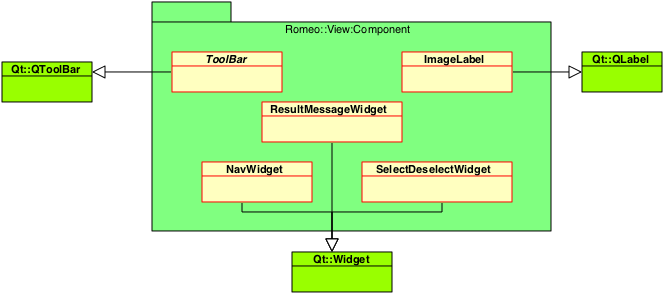
\includegraphics[width=\linewidth]{../Specifica_Tecnica/Content/Immagini/Romeo__View__Component.png}
			\caption{Componente Romeo::View::Component}
			\label{comp_romeo::view::component}
\end{figure}
\pagebreak
%%%%%%%%%%%%%%%%%%%
% 	TOOLBAR
%%%%%%%%%%%%%%%%%
\subsubsection{ToolBar(class)}
\label{spetool}
\begin{figure}[!h]
\centering
			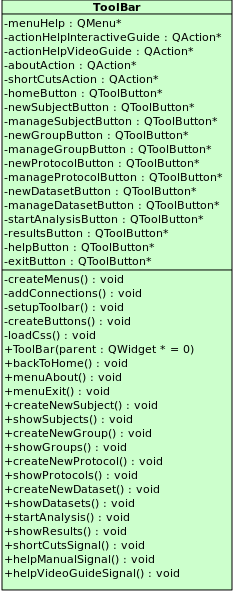
\includegraphics[width=0.65\linewidth]{./Content/Immagini/view/ToolBar.png}
			\caption{Classe ToolBar: attributi e metodi}
			\label{cl_tool}
\end{figure}
\paragraph{Descrizione \\}
Classe che rappresenta la componente contenuta nelle finestre per poter filtrare i contenuti delle tabelle presentei nella vista in base a diversi parametri secondo le preferenze dell'utente.
\paragraph{Utilizzo\\}
La classe viene utilizzata per dare all'utente la possibilità di visualizzare i dati tabellari ordinandoli secondo una certa caratteristica scelta dall'utente nel momento in cui si trova sulla finestra che espone una tabella.
\paragraph{Classi ereditate\\}
\begin{itemize}
\item Qt::QWidget.
\end{itemize}
%%%%%%%%%  METODI
\paragraph{\textcolor{black}{Metodi\\}}
%costruttore
\color{blue}\verb! + ToolBar(parent : QWidget*=0)!
\begin{quote}
\color{black}Costruttore per la classe ToolBar. \\
\textbf{Argomenti}
\begin{itemize}
\item parent: QWidget*=0  \\ Puntatore al QWidget padre di ToolBar.
\end{itemize}
\end{quote}
%crateToolBar()
\color{blue}\verb! +CreateToolBar():void!
\color{black}
\begin{quote}

\end{quote} 
\color{black}
\pagebreak
%%%%%%%%%%%%%%%%%%
%	SELECTDESELECT
%%%%%%%%%%%%%%%%%%
\subsubsection{SelectDeselectWidget (class)}
\label{speselDes}
\begin{figure}[!h]
\centering
			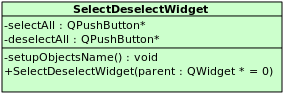
\includegraphics[width=0.6\linewidth]{./Content/Immagini/view/SelectDeselectWidget.png}
			\caption{Classe SelectDeselectWidget: attributi e metodi}
			\label{cl_seldesel}
\end{figure}
\paragraph{Descrizione \\}
Classe che rappresenta la componente che permette, dove previsto, di velocizzare le operazioni dell'utente qualora voglia selezionare (o deselezionare) l'intero insieme dei dati.
\paragraph{Utilizzo\\}
La classe viene utilizzata dalle viste che presentano un elenco di dati, che l'utente può selezionare per poi compiere determinate azioni sugli elementi scelti. È molto utile quando l'utente ha da selezionare (rispettivamente, deselezionare) un numero molto alto di voci.
\paragraph{Classi ereditate\\}
\begin{itemize}
\item Qt::QWidget.
\end{itemize}
%%%%%%%%%%%%%%ATTRIBUTI%%%%%%%%%%%
\paragraph{\textcolor{black}{Attributi\\}}
\color{teal}\verb!-selectAll: QPushButton*!
\begin{quote}
\color{black}Pulsante che permette la selezione contemporanea di tutte le voci della tabella.
\end{quote}
\color{teal}\verb!-deselectAll: QPushButton*!
\begin{quote}
\color{black}Pulsante che permette la deselezione contemporanea di tutte le voci della tabella.
\end{quote}
%%%%%%%%%  METODI
\paragraph{\textcolor{black}{Metodi\\}}
%costruttore
\color{blue}\verb! + SelectDeselectWidget(parent : QWidget*=0)!
\begin{quote}
\color{black}Costruttore per la classe SelectDeselectWidget. \\
\textbf{Argomenti}
\begin{itemize}
\item parent: QWidget*=0  \\ Puntatore al QWidget padre di ToolBar.
\end{itemize}
\end{quote}
%setupObjName()
\color{blue}\verb! -setupObjectName():void!
\color{black}
\begin{quote}Metodo che ha il compito di impostare i nomi degli oggetti contenuti all'interno del widget \emph{SelectDeselectAll}.
\end{quote} 
\color{black}
\pagebreak
%%%%%%%%%%%%%%%%
%	NAVWIDGET
%%%%%%%%%%%%%%%%
\subsubsection{NavWidget (class)}
\label{spenav}
\begin{figure}[!h]
\centering
			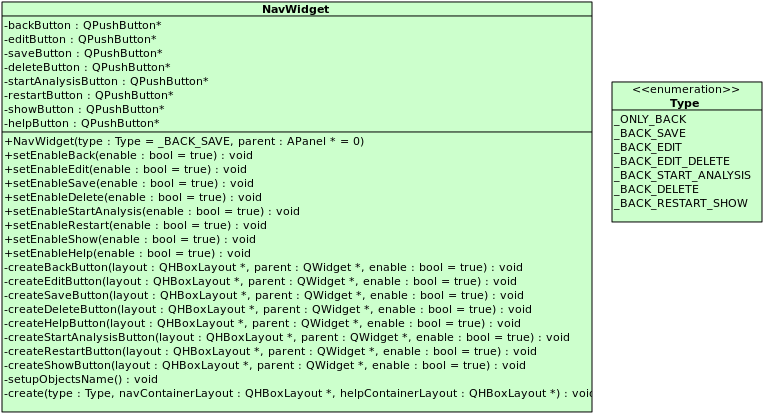
\includegraphics[width=1.1\linewidth]{./Content/Immagini/view/NavWidget.png}
			\caption{Classe NavWidget: attributi e metodi}
			\label{cl_nav}
\end{figure}
\paragraph{Descrizione \\}
Classe che rappresenta la componente disposta nella parte bassa del layout della finestra contenente i pulsanti per la navigazione all'indietro, la visualizzazione della guida interattiva e, ove previsti, i pulsanti per la modifica, per la cancellazione e per il salvataggio delle modifiche apportate.
\paragraph{Utilizzo\\}
La classe viene utilizzata da tutte le viste in quanto è sicuramente sempre presente il pulsante per ritornare alla finestra precedente e per l'apertura della guida; gli altri pulsanti saranno presenti ove vi è la possibilità di effettuare operazioni che influiscono sullo stato del sistema come per esempio l'inserimento di un nuovo \subject{} o la cancellazione di un \protocol{} o ancora la modifica di un gruppo di \subject{}.
\paragraph{Classi ereditate\\}
\begin{itemize}
\item Qt::QWidget.
\end{itemize}
%%%%%%%%%%%%%%ATTRIBUTI%%%%%%%%%%%
\paragraph{\textcolor{black}{Attributi\\}}
\color{teal}\verb!-backButton: QPushButton*!
\begin{quote}
\color{black}Pulsante che permette il ritorno alla finestra precedente.
\end{quote}
\color{teal}\verb!-editButton: QPushButton*!
\begin{quote}
\color{black}Pulsante che permette la modifica di alcuni dati visualizzati nella vista.
\end{quote}
\color{teal}\verb!-saveButton: QPushButton*!
\begin{quote}
\color{black}Pulsante che permette il salvataggio delle modifiche precedentemente effettuate.
\end{quote}
\color{teal}\verb!-deleteButton: QPushButton*!
\begin{quote}
\color{black}Pulsante che permette la rimozione degli oggetti selezionati.
\end{quote}
\color{teal}\verb!-helpButton: QPushButton*!
\begin{quote}
\color{black}Pulsante che permette la visualizzazione della guida interattiva.
\end{quote}
\color{teal}\verb!-startButton: QPushButton*!
\begin{quote}
\color{black}Pulsante che permette di avviare una nuova analisi.
\end{quote}
%%%%%%%%%  METODI
\paragraph{\textcolor{black}{Metodi\\}}
%costruttore
\color{blue}\verb! + NavWidget(type: Type, parent : QWidget*=0)!
\begin{quote}
\color{black}Costruttore per la classe NavWidget. \\
\textbf{Argomenti}
\begin{itemize}
\item type: Type \\ suggerisce la tipologia di NavWidget da costruire:
\begin{itemize}
\item solo ritorno alla finestra precedente e visualizzazione guida (es. visualizzazione \subject{} presenti nel sistema);
\item ritorno alla finestra precedente e salvataggio operazioni (es. per le viste che si occupano di creare nuovi elementi);
\item ritorno alla finestra precedente e possibilità di modifica dei campi (es. visualizzazione gruppi di \subject{});
\item ritorno alla finestra precedente e possibilità di cancellare elementi selezionati (es. visualizzazione \protocol{});
\item ritorno alla finestra precedente e possibilità di avviare l'analisi (es. starAnalysis).
\end{itemize}
\item parent: QWidget*=0  \\ Puntatore al QWidget padre di ToolBar.
\end{itemize}
\end{quote}
%setupObjName()
\color{blue}\verb!-setupObjectName():void!
\color{black}
\begin{quote}Metodo che ha il compito di impostare i nomi degli oggetti contenuti all'interno del widget \emph{SelectDeselectAll}.
\end{quote} 
\color{black}
%createBackButton
\color{blue}\verb!-createBackButton(layout:QHBoxLayout*, parent:QWidget*= 0, enable:bool= true): void!
\color{black}
\begin{quote}Metodo che ha il compito di creare il campo dati \emph{backButton}.\\
\textbf{Argomenti}
\begin{itemize}
\item layout: QHBoxLayout* \\ box per dare un'allineamento orizzontale del pulsante;
\item parent: QWidget*=0  \\ Puntatore al QWidget padre di NavWidget;
\item enable: bool=true \\ caratteristica del pulsante ad essere abilitato alla pressione, di default è true.
\end{itemize}
\end{quote}
%createEditButton
\color{blue}\verb!-createEditButton(layout:QHBoxLayout*, parent:QWidget*=0, enable:bool=true):void!
\color{black}
\begin{quote}Metodo che ha il compito di creare il campo dati \emph{editButton}.\\
\textbf{Argomenti}
\begin{itemize}
\item layout: QHBoxLayout* \\ box per dare un'allineamento orizzontale del pulsante;
\item parent: QWidget*=0  \\ Puntatore al QWidget padre di NavWidget;
\item enable: bool=true \\ caratteristica del pulsante ad essere abilitato alla pressione, di default è true.
\end{itemize}
\end{quote}
%createSaveButton
\color{blue}\verb!-createSaveButton(layout:QHBoxLayout*, parent:QWidget*=0, enable:bool= true):void!
\color{black}
\begin{quote}Metodo che ha il compito di creare il campo dati \emph{saveButton}.\\
\textbf{Argomenti}
\begin{itemize}
\item layout: QHBoxLayout* \\ box per dare un'allineamento orizzontale del pulsante;
\item parent: QWidget*=0  \\ Puntatore al QWidget padre di NavWidget;
\item enable: bool=true \\ caratteristica del pulsante ad essere abilitato alla pressione, di default è true.
\end{itemize}
\end{quote} 
%createdeleteButton
\color{blue}\verb!-createDeleteButton(layout:QHBoxLayout*, parent:QWidget*=0, enable:bool=true):void!
\color{black}
\begin{quote}Metodo che ha il compito di creare il campo dati \emph{deleteButton}.\\
\textbf{Argomenti}
\begin{itemize}
\item layout: QHBoxLayout* \\ box per dare un'allineamento orizzontale del pulsante;
\item parent: QWidget*=0  \\ Puntatore al QWidget padre di NavWidget;
\item enable: bool=true \\ caratteristica del pulsante ad essere abilitato alla pressione, di default è true.
\end{itemize}
\end{quote}
%createHelpButton
\color{blue}\verb!-createHelpButton(layout:QHBoxLayout*, parent:QWidget*=0, enable:bool=true):void!
\color{black}
\begin{quote}Metodo che ha il compito di creare il campo dati \emph{helpButton}.\\
\textbf{Argomenti}
\begin{itemize}
\item layout: QHBoxLayout* \\ box per dare un'allineamento orizzontale del pulsante;
\item parent: QWidget*=0  \\ Puntatore al QWidget padre di NavWidget;
\item enable: bool=true \\ caratteristica del pulsante ad essere abilitato alla pressione, di default è true.
\end{itemize}
\end{quote}
%createStartButton
\color{blue}\verb!-createStartAnalysisButton(layout:QHBoxLayout*, parent:QWidget*=0, enable:bool=true):void!
\color{black}
\begin{quote}Metodo che ha il compito di creare il campo dati \emph{startButton}.\\
\textbf{Argomenti}
\begin{itemize}
\item layout: QHBoxLayout* \\ box per dare un'allineamento orizzontale del pulsante;
\item parent: QWidget*=0  \\ Puntatore al QWidget padre di NavWidget;
\item enable: bool=true \\ caratteristica del pulsante ad essere abilitato alla pressione, di default è true.
\end{itemize}
\end{quote}
\color{black}
\pagebreak
%%%%%%%%%%%%%%%%%%%%%%%%%%
%	 menuBar
%%%%%%%%%%%%%%%%%%%%%%%%%
\subsubsection{MenuBar (class)}
\label{spemenu}
\begin{figure}[!h]
\centering
			\includegraphics[width=0.4\linewidth]{./Content/Immagini/view/MenuBar.png}
			\caption{Classe NavWidget: attributi e metodi}
			\label{cl_nav}
\end{figure}
\paragraph{Descrizione \\}
Classe che rappresenta la componente barra del menu che contiene tutte le azioni che l'utente può fare. È presente nella finestra principale del programma.
\paragraph{Utilizzo\\}
La classe viene utilizzata dalla classe \emph{MainWindow}	 e fornisce un rapido accesso alle funzionalità di \project{}.
\paragraph{Classi ereditate\\}
\begin{itemize}
\item Qt::QMenuBar.
\end{itemize}
%%%%%%%%%%%%%%ATTRIBUTI%%%%%%%%%%%
\paragraph{\textcolor{black}{Attributi\\}}
\color{teal}\verb!-menuNew: QMenu*!
\begin{quote}
\color{black} Rappresenta il menu per la creazione di un elemento.
\end{quote}
%menuShow
\color{teal}\verb!-menuShow: QMenu*!
\begin{quote}
\color{black} Rappresenta il menu per la visualizzazione degli elementi presenti in \project{}.
\end{quote}
%menuAnalysis
\color{teal}\verb!-menuAnalysis: QMenu*!
\begin{quote}
\color{black} Rappresenta il menu per l'esecuzione di una nuova analisi.
\end{quote}
%menuHelp
\color{teal}\verb!-menuHelp: QMenu*!
\begin{quote}
\color{black} Rappresenta il menu per la visualizzazione della guida interattiva.
\end{quote}
%%%%%%%%%%%%%%%%%%%% ACTION
%actNewSub
\color{teal}\verb!-actionNewSubject: QAction*!
\begin{quote}
\color{black} Voce contenuta in \emph{menuNew} e porta alla finestra per la creazione di un nuovo \subject{}.
\end{quote}
%actNewGroup
\color{teal}\verb!-actionNewGroup: QAction*!
\begin{quote}
\color{black} Voce contenuta in \emph{menuNew} e porta alla finestra per la creazione di un nuovo gruppo di  \subject{}.
\end{quote}
%actNewprotocol
\color{teal}\verb!-actionNewProtocol: QAction*!
\begin{quote}
\color{black} Voce contenuta in \emph{menuNew} e porta alla finestra per la creazione di un nuovo \protocol{}.
\end{quote}
%actNewDataset
\color{teal}\verb!-actionNewDataset: QAction*!
\begin{quote}
\color{black} Voce contenuta in \emph{menuNew} e porta alla finestra per la creazione di un nuovo \dataset{}.
\end{quote}
%%%%%%%%% show %%%%%%%%%%%%5
%actshowSub
\color{teal}\verb!-actionShowSubjects: QAction*!
\begin{quote}
\color{black} Voce contenuta in \emph{menuShow} e porta alla finestra per la visualizzazione dei \subject{} presenti nel sistema.
\end{quote}
%actShowGroup
\color{teal}\verb!-actionShowGroups: QAction*!
\begin{quote}
\color{black} Voce contenuta in \emph{menuShow} e porta alla finestra per la visualizzazione dei gruppi di \subject{} presenti nel sistema.
\end{quote}
%actshowprotocol
\color{teal}\verb!-actionShowProtocols: QAction*!
\begin{quote}
\color{black} Voce contenuta in \emph{menuShow} e porta alla finestra per visualizzazione dei \protocol{} presenti nel sistema.
\end{quote}
%actshowDataset
\color{teal}\verb!-actionShowDatasets: QAction*!
\begin{quote}
\color{black} Voce contenuta in \emph{menuShow} e porta alla finestra per la visualizzazione dei \dataset{} presenti nel sistema.
\end{quote}
%statAnalysis
\color{teal}\verb!-actionAnalysisStart: QAction*!
\begin{quote}
\color{black} Voce contenuta in \emph{menuAnalysis} e porta alla finestra per l'avvio di una nuova analisi.
\end{quote}
%ResultsAnalysis
\color{teal}\verb!-actionAnalysisResults: QAction*!
\begin{quote}
\color{black} Voce contenuta in \emph{menuAnalysis} e porta alla finestra per la visualizzazione dei risultati delle analisi presenti in \project{}.
\end{quote}
%guidaInterattiva
\color{teal}\verb!-actionHInteractiveGuide: QAction*!
\begin{quote}
\color{black} Voce contenuta in \emph{menuHelp} e apre la finestra di dialogo contentente la guida interattiva che l'utente può consultare.
\end{quote}
%about
\color{teal}\verb!-actionAbout: QAction*!
\begin{quote}
\color{black} Voce che apre la finestra contenente le informazioni relative agli sviluppatori di \project{}.
\end{quote}
%Exit
\color{teal}\verb!-actionExit: QAction*!
\begin{quote}
\color{black} Voce che permette di uscire dall'applicativo \project{}.
\end{quote}
%%%%%%%%%%% METODI %%%%%%
\paragraph{\textcolor{black}{Metodi\\}}
%costruttore
\color{blue}\verb! + MenuBar()!
\begin{quote}
\color{black}Costruttore per la classe MenuBar. \\
\end{quote}
%setupObjName()
\color{blue}\verb! -setupObjectName():void!
\color{black}
\begin{quote}Metodo che ha il compito di impostare i nomi degli oggetti contenuti all'interno del widget \emph{SelectDeselectAll}.
\end{quote}
%addConnect
\color{blue}\verb! -addConnection(): void!
\color{black} 
\begin{quote}
Metodo che ha il compito di fissare tutte le istruzioni \emph{connect} degli oggetti che emetteranno un signal\g{} verso il rispettivo controller.
\end{quote} 
%setActions
\color{blue}\verb! -setActions(): void!
\color{black} 
\begin{quote}
Metodo che ha il compito di impostare le action ai campi dati di tipo \emph{QAction*}.
\end{quote} 
\color{black}
%setMenus
\color{blue}\verb! -setMenus(): void!
\color{black} 
\begin{quote}
Metodo che ha il compito di impostare le voci del MenuBar.
\end{quote} 
%setMenuBar
\color{blue}\verb! -setMenuBar(): void!
\color{black} 
\begin{quote}
Metodo che ha il compito di impostare la MenuBar.
\end{quote} 
%addCo
\color{blue}\verb! -addActionsToMenus(): void!
\color{black} 
\begin{quote}
Metodo che aggiunge le voci ai vari menu.
\end{quote} 
%%%%%%%%%%%%%%% SIGNALS
%menuabout
\color{blue}\verb! +menuAbout():void! (signal)
\color{black} 
\begin{quote}
Signal\g{} emesso quando l'utente seleziona la voce \emph{About} dalla barra del menu.
\end{quote}
%menuEx
\color{blue}\verb! +menuExit():void! (signal)
\color{black} 
\begin{quote}
Signal\g{} emesso quando l'utente seleziona la voce \emph{Exit} dalla barra del menu per chiudere l'applicazione.
\end{quote}
%createNewSub
\color{blue}\verb! +createNewSubject():void! (signal)
\color{black} 
\begin{quote}
Signal\g{} emesso quando l'utente seleziona da \emph{MenuNew} la voce \emph{Subject}.
\end{quote}
%showSubs
\color{blue}\verb! +showSubjects():void! (signal)
\color{black} 
\begin{quote}
Signal\g{} emesso quando l'utente seleziona da \emph{MenuShow} la voce \emph{Subjects}.
\end{quote}

%createNewgr
\color{blue}\verb! +createNewGroup():void! (signal)
\color{black} 
\begin{quote}
Signal\g{} emesso quando l'utente seleziona da \emph{MenuNew} la voce \emph{Group}.
\end{quote}
%showgroups
\color{blue}\verb! +showGrops():void! (signal)
\color{black} 
\begin{quote}
Signal\g{} emesso quando l'utente seleziona da \emph{MenuShow} la voce \emph{Groups}.
\end{quote}

%createNewProtocol
\color{blue}\verb! +createNewProtocol():void! (signal)
\color{black} 
\begin{quote}
Signal\g{} emesso quando l'utente seleziona da \emph{MenuNew} la voce \emph{Protocol}.
\end{quote}
%showProtocols
\color{blue}\verb! +showProtocols():void! (signal)
\color{black} 
\begin{quote}
Signal\g{} emesso quando l'utente seleziona da \emph{MenuShow} la voce \emph{Protocols}.
\end{quote}

%createNewdata
\color{blue}\verb! +createNewDataset():void! (signal)
\color{black} 
\begin{quote}
Signal\g{} emesso quando l'utente seleziona da \emph{MenuNew} la voce \emph{Dataset}.
\end{quote}
%showSubs
\color{blue}\verb! +showDatasets():void! (signal)
\color{black} 
\begin{quote}
Signal\g{} emesso quando l'utente seleziona da \emph{MenuShow} la voce \emph{Datasets}.
\end{quote}


%start
\color{blue}\verb! +startAnalysis():void! (signal)
\color{black} 
\begin{quote}
Signal\g{} emesso quando l'utente seleziona da \emph{MenuAnalysis} la voce \emph{Start}.
\end{quote}
%showSubs
\color{blue}\verb! +showResults():void! (signal)
\color{black} 
\begin{quote}
Signal\g{} emesso quando l'utente seleziona da \emph{MenuAnalysis} la voce \emph{Result}.
\end{quote}